\subsection{BeagleBone Black} % 
		\subsubsection{Background} % Hampus
The BeagleBone Black (BBB) is a single board computer with a 1GHz single core ARM processor and 512 MB of RAM. It is the hardware that is most similar to a desktop environment in Naiad which makes it more convenient to place the more abstract software on. The software however can not be cross compiled as there is no proper cross compiler for Ada. This means that all code has to be natively compiled on a ARM architecture, where the BBB itself is generally the most convenient. The BBB supports CAN but because the limitation of using 3.3V for logical input and output compared to 22-24V on the CAN-bus. It is instead connected to a CAN-card via UART which translates all of the CAN messages. The UART on a CAN-card is however using 5V logic, this is solved with a simple bi-directional level shifter converter. The operating system is a scaled down, prepackaged armhf\cite{armhf} version of Ubuntu. It only requires around 400MB which makes it possible to only require the on board 2GB flash for operating system and software.

		\subsubsection{PID-controller} % Joakim
\noindent 
One Proportional Integration Derivative (PID) and five PD controllers was implemented in the Naiad robot to control the position and orientation to achieve desired state of the robot.
\subsubsection*{State estimation}
The initial state of the robot sets the global space coordinate system that will act as a reference frame under the runtime. The robot in it self has its own reference coordinate system which is the local space of the robot that all the motor calculations will be calculated in.

Since it is hard to get a good estimation of the position by integrating the acceleration data the positional estimation was neglected and the IMU was only used to get the roll, pitch and yaw angles which were more accurate and their estimated values did not drift.

\subsubsection*{Error calculation}
\noindent 
The PD/PID controller bases its control values on the difference (error) between the desired and the current state of the robot. This error is handled as a vector that contains the error of the positional and the orientational states of the robot, see fig. \ref{pid_pic}. 


\begin{figure}[!ht]
\begin{center}
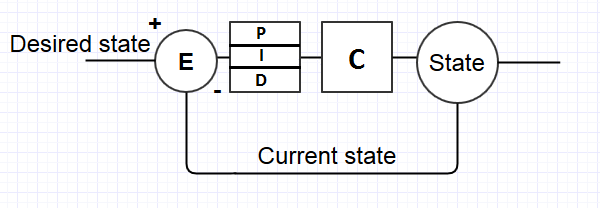
\includegraphics[width=80mm]{./Images/Software/simplepid.png}
\\
\caption{\label{pid_pic}Simplified PID control loop}
\end{center}
\end{figure}


Since the natural floating of the robot gives a stable horizontal orientation the most important factor of the orientation is to get a proper planar motion. This is done by keeping track of the angle around the Z axis, the yaw angle.

By keeping the position and orientation data relative to the starting state of the robot, it is possible to calculate which motors should be activated and how much depending on the current state of the robot. This is done by transferring the desired state that is given in global space coordinates into coordinates of the robots local space.

When the difference between the desired state and the current state is determined the control values that represent the desired speed of the motors can be determined by the equations \ref{pid_eq1}-\ref{pid_eq2}.

\begin{center}
\begin{figure}[!ht]
\begin{equation}
O_{error}=O_{desired}-O_{current}
\label{pid_eq1}
\end{equation}
\begin{equation}
XY_{error}=XY_{desired}-XY_{current}
\end{equation}
\begin{equation}
Depth_{error}=Depth_{desired}-Depth_{current}
\end{equation}
\begin{equation}
O_{p}=K_{p}*O_{error}
\end{equation}
\begin{equation}
O_{d}=K_{d}*(O_{error} - O_{previous})
\end{equation}
\begin{equation}
XY_{p}=K_{p}*XY_{error}
\end{equation}
\begin{equation}
XY_{d}=K_{d}*(XY_{error} - XY_{previous})
\end{equation}
\begin{equation}
Depth_{p}=K_{p}*Depth_{error}
\end{equation}
\begin{equation}
Depth_{i}=Depth_{i} + K_{i}*Depth_{error}*dt
\end{equation}
\begin{equation}
Depth_{d}=K_{d}*(Depth_{error} - Depth_{previous})
\end{equation}
\caption{Error equations}
\end{figure}
\end{center}


\begin{center}
\begin{figure}[!ht]
\begin{equation}
O_{output}=O_{p}+O_{d}
\end{equation}
\begin{equation}
XY_{output}=XY_{p}+XY_{d}
\end{equation}
\begin{equation}
Depth_{output}=Depth_{p}+Depth_{i}+Depth_{d}
\label{pid_eq2}
\end{equation}
\caption{Control values}
\end{figure}
\end{center}

The control values are added and multiplied with the corresponding motion component of each motor which gives a motor value between 0 and 255 where a value below 128 means that the motor is going backwards and a value higher than 128 means it is going forward. The calculated motor speeds is then sent to the CAN node that sends the values to corresponding motor controller.

		\subsubsection{Sensor fusion} % Wenkai
		\noindent

		The sensor fusion is aimed to calculate the attitude which include yaw, pitch, roll and integrate the accelerate value of x, y and z twice to get the origin position. Since the value of the pitch, roll and accelerometer z value from the IMU are good enough, so about the sensor fusion part now is mainly focus on the accelerometer x and accelerometer y.
	The accelerometer X value and accelerometer Y value that comes from the IMU have a lot of noise. This makes it is quite hard for the NAIAD to go straight and do other tasks. The integration of the accelerometer value is the velocity value, and the integration of the velocity value is the distance. As can be seen after integration twice, the small noise from the accelerometer can become very big. This will lead Naiad to not be able to get the correct distance value. Even though there is a Kalman filter in the IMU device, but the accelerometer value x and y still have a lot of noise, that is quite bad. Now we let the value go through the Kalman filter that we build again.
		\subsubsection*{Sensor fusion calculation by using Kalman Filter}
		\noindent
		First here is some basic knowledge about Kalman filter, it is a very powerful tool when trying to controlling a noisy system\cite{kalman_filter}.In 'A practical approach to Kalman filter and how to implement it' it is written that "The Kalman filter will then try to estimate the state of the system, based on the current and previous states, that tend to be more precise that than the measurements alone."\cite{TKJ} Kalman Filter is discrete, it rely on measured samples taken between repeated but constant periods of time. This means that the result is approximated good enough, but there is something that can't be known between the samples\cite{Greg_Czerniaks_Website} and \cite{change_parameter}. The soul of the Kalman filter is the five equations which is shown below:
\begin{equation}
\label{wenkai1}
	X_{k|k-1} = A*X_{k-1|k-1} +B*u_{k}
\end{equation}
\begin{equation}
\label{wenkai2}
	P_{k|k-1} = A*P_{k-1|k-1}*A^{T} + Q
\end{equation}
The equation \ref{wenkai1} and \ref{wenkai2} above are Time update which means they are the prediction value for the next round calculate.
\begin{equation}
\label{wenkai3}
K_{g} = P_{k|k-1}*H^{T}/(H*P_{k|k-1}*H^{T}+R)
\end{equation}
\begin{equation}
\label{wenkai4}
	X_{k|k} = X_{k|k-1} +K_{g}*(Z_{k}-H*X_{k|k-1})
\end{equation}
\begin{equation}
\label{wenkai5}
P_{k|k}=(I-Kg_{k}* H)*P_{k|k-1}
\end{equation}
 The equations \ref{wenkai3} to \ref{wenkai5} are measurement update. These updated values will correct the value that is wanted\cite{kalman_filter_dummies}. About the parameters of A,B,P,H,Q,R,K, more details will be found in\cite{parameter}.
 For now the Kalman filter which depends on Naiad can be built from a mathematics model system. The parameters is set manually like P = 1000.0, Q = 0.01 and R = 0.1. When Naiad is kept on a table, the accelerometer x and y value suppose to be 0, but the real value is not 0, so this value is set as the error value. The average error is calculated and then removed. When integrating the accelerometer value to get the velocity, the velocity value still not 0. The average error is recalculated and removed again. After that the velocity is quite small. Now if the absolute value of velocity is in the range 0 to 0.5E-03, then the velocity is set to 0, otherwise remove 0.5E-03 from the value. When the velocity value is integrated the distance is good enough to be used.

		\subsubsection{Mission control} % Jonatan
		\noindent Since each mission is more or less unique, a routine for each is needed.
		Most of the missions gets feedback from sensors and then update the relative coordinates for the PID-controller or if an action should be needed, for example fire torpedo.
		It is heavily depending on the data from vision in form of a distance vector to the object or objects that is interesting for completing the mission.
		
		\subsubsection{Path planning} % Jonatan
		\noindent Path planning in water differs from other mediums due to the special characteristics of water. The more static environment and the ability to move freely in three dimensions reduces the complexity of navigate without obstacles interfere with the path. For these reasons a simple path planner was implemented for the main purpose to aid the PID-controller by splitting movement to smaller parts which ensures that the proportional part of the controller doesn't exceeds the maximum values for the motors, which would make control of the unit close to impossible. 
		
				\subsubsection{Side scan sonar} % Jonatan
		\noindent The side scan sonar \cite{side_scan_sonar} sends out a sound then measuring the effect received, over 60 degrees split in to 1000 points with 1 byte resolution for up to 25 meters distance. This can in the future be a huge asset when it comes to aiding the vision system or to gain some more knowledge about an objects.


\subsubsection{Can node translator} % Hampus
\noindent The CAN node is a simple node that is translating messages between Ethernet and CAN. All of the received Ethernet messages with the correct structures will be translated into CAN messages which is sent to the CAN-bus via UART to a CAN-card. All of the expected incoming CAN messages must be predefined to know where the message should be sent. The CAN node does also convert data that have been split because of the limited eight single bytes structure of the data in CAN messages. Due to the nature of UART the node uses busy waiting to read the data. To reduce the CPU usage, the node goes to sleep for a moment while the UART buffer is empty. This means that a message sent from a CAN-card might be slightly delayed in a BBB's buffer.


\subsubsection{Border Gateway} % Hampus
\noindent The TCP communication is based on a server – client structure. The server will act as a central node and be a gateway to all of the other nodes. This makes it simple to decide where messages should be sent as it can just be specified in the messages itself, not requiring a client to be directly connected with the node it wants to talk to. A drawback is that all the messages has to be sent twice, effectively doubling the number of messages on the network. This also means that each client only needs one open connection which is to the server. All but the initial communication is based on JavaScript Object Notation (JSON). So all messages contains variables with variable names expressed as a string. This allows a simple and compressed way to send data structure over TCP between programs written in different languages. A drawback is that variable names in the structure have to be predefined in some languages which makes it less dynamic. 

To initiate a full connection to the server, a client has to first connect to a predefined port that is the same for all clients. When a client is connected on that port, the server expects a message containing a string of three characters. The string is important as the server will use that as the reference name for that connection and pass all messages that targets that name to that connection. After the initial string is received, it will first check if that name already have connected in which case it will do nothing but drop the current connection. If it is a new connection, the server will connect to an internal thread and pass the name on. The server has a predefined number of threads that will be ready to handle connections. When a thread receives a name, it will open a server connection and wait on a port that is related to the name itself. The port number is calculated by using the each letters as a number in base 26. It makes the possible port range go from 0 (aaa) to 17576 (zzz), depending on the name. When the client connects to the new connection, the initial set-up connection is done. A thread that is now handling a connection will sit and wait for an incoming message of the size 256 bytes. This is done to simplify and speed up the handling of messages as the alternative is to either read every single byte to check for termination sign or to always start a message by sending a single integer that will tell the size of the following message. In the message itself, there should be a JSON variable called 'target' containing a three character long string with the name. This will tell the server where it should send the message. If the variable does not exist or if the target name have not connected yet, the message will be thrown away. 

After an initial connection is established at least once, there is no requirement to reinitialize the connection if the connection would drop, as the server connection will reset on that port, but it will also not do any harm. This also means that a specific thread will never change it's port after it has been set. Because the server is running on a Linux operating system, it is configured to use the keepalive setting on the TCP connection which will probe to see if the connection have been physically disconnected. The keepalive timer is depended on a setting in the operating system, the default time before checking is 7200 seconds. The current timer is set to detect a broken physical connection after around 3 seconds. Other connection issues can trigger a detection of a client drop much faster. It does not have any timeout settings enabled, so it will never drop the client by itself. The maximum number of clients is currently 20. The server will never be busy waiting as when it waits for a connection or when it is waiting for a message, it will sleep until it is awaken by an interrupt from the operating system due to activity on the Ethernet. This will only happen if the buffer is filled, which is if it receives 256 bytes. The server does also support the ability to mirror or/and disable traffic to nodes. All that is required to set the server node as the message target, set a variable name to 'ethid' 2 or 3 respectively and send boolean with a variable names of the target node where the traffic should be manipulated. Note that on some operating systems, opening a port requires higher user privileges, for example by using sudo on a Linux operating system.

